\documentclass{article}
\usepackage{graphicx} % Required for inserting images

\title{DevOps24-groupK\\
\large Course Code: BSDSESM1KU}
\author{GitGurus}
\date{Spring 2024}

% \usepackage{graphicx} % Required for inserting images
% \usepackage{amsmath}
% \usepackage{hyperref}
\usepackage{listings}
\lstset
{
    basicstyle=\footnotesize,
    numbers=left,
    stepnumber=1,
    showstringspaces=false,
    tabsize=1,
    breaklines=true,
    breakatwhitespace=false,
}

\usepackage[utf8]{inputenc}
\usepackage[T1]{fontenc}
\usepackage[english]{babel}
\usepackage{minted}
% \usepackage[a4paper, bottom=3cm, top=3cm, left=2.5cm, right=2.5cm]{geometry}
\usepackage[linewidth=1pt]{mdframed}
\usepackage{ebproof}
\usepackage{amsmath}
% \usepackage{fourier}
\usepackage{booktabs}
% \usepackage{inconsolata}
\usepackage{float}
\usepackage{lastpage}
\usepackage{graphicx}
\usepackage{titling}
\usepackage{fancyhdr}
\usepackage[dvipsnames]{xcolor}
\usepackage[hidelinks]{hyperref}

\renewcommand{\baselinestretch}{1.2} % Line spacing
% \setlength{\parindent}{0em} % Paragraph indent
% \setlength{\parskip}{0.75em} % Paragraph vertical spacing

% \colorlet{LightGray}{Gray!7!}

% % global minted styles
% \setminted{bgcolor=LightGray, breaklines, frame=single, linenos, fontsize=\small, numbersep=8pt}

% % minted remove red squares around "erroneus" code
% \AtBeginEnvironment{minted}{%
%   \renewcommand{\fcolorbox}[4][]{#4}}

% % minted line number style
% \renewcommand{\theFancyVerbLine}{{\scriptsize \arabic{FancyVerbLine}}}
\begin{document}

\maketitle

\begin{table}[H]
    \centering
    \begin{tabular}{c|c}
    Andreas Guldborg Hansen & aguh@itu \\
    Andreas Severin Hauch Trøstrup & atro@itu.dk \\
    Frederik Petersen & frepe@itu.dk \\
    Mads Aqqalu Roager & mroa@itu.dk \\
    Silke Holme Bonnen & ssbo@itu.dk
    \end{tabular}
\end{table}

\newpage
\tableofcontents

\newpage


\section{Systems' perspective}
\subsection{Design and architecture}
An overview of the architecture of our MiniTwit application can be found in figure \ref{fig:architecture}. 
The entire system runs on DigitalOcean, with the exception of our monitoring and logging that runs on New Relic.
In DigitalOcean, we have 3 primary nodes running. A swarm manager, and two workers. These 3 nodes are a part of a docker swarm network that runs the minitwit web app and minitwit simulator API containers as docker services.
The workers and manager also run a New Relic agent that collects logs and system monitoring information, and send it to new relic.
The manager node runs a Nginx reverse proxy, that handles https encryption, and load balancing between the workers.
Lastly, in DigitalOcean we also have a managed database running, that acts as the database for the application.
What the diagram below does not show is that the swarm manager also has a container running the web app and the simulator API. The reason why this is not shown on the diagram is because the Nginx reverse proxy has been set to only forward requests to worker 1 and 2. 
That means that the web app and the simulator api in the swarm manager will never be used. 


\begin{figure}[H]
    \centering
    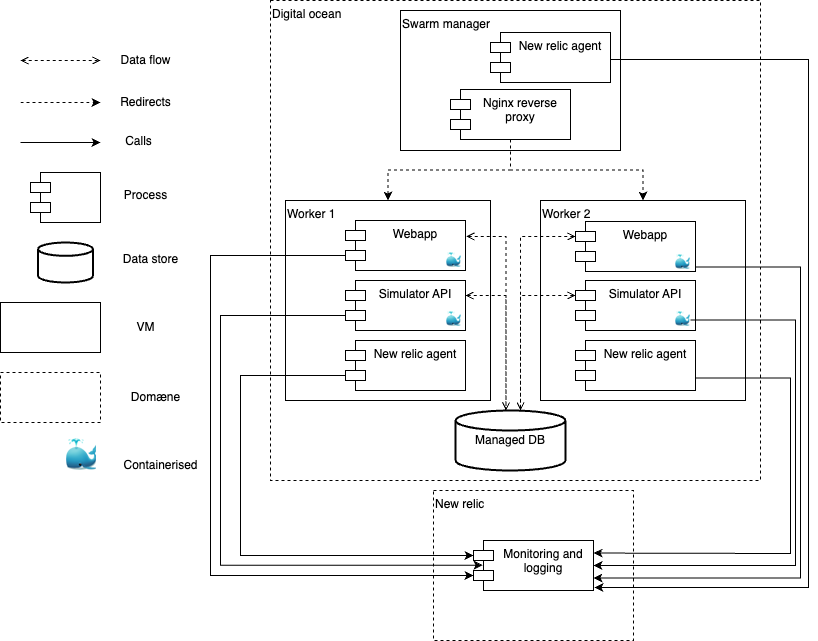
\includegraphics[width=\textwidth]{images/devops-overview.png}
    \caption{The figure shows a diagram of the architecture of minitwit}
    \label{fig:architecture}
\end{figure}

\subsection{Dependencies}
Our application has numerous dependencies, so we have priorities to describe the dependencies that are critical to our application in production. That is, if there is a problem with one of these dependencies, e.g. a dependency has a open security problem, then we have a problem. 

In the dependency graph, available in Figure \ref{fig:dep-prod}, only the direct dependencies in production is shown. There is one exception to this, PostgreSQL is shown as a dependency to DigitalOcean. We decided that it was important to show this dependency as it is a critical dependency for our application.
Besides from this, we do not show what our dependencies depend on and we do not show the development dependencies. The most important development dependencies can be seen in appendix \ref{appendix: dev-dependecies}.

\begin{figure}[H]
    \centering
    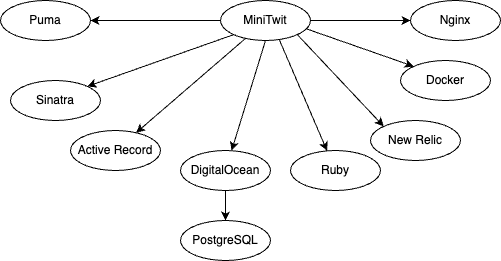
\includegraphics[width=0.8\textwidth]{images/dependency-graph-prod.png}
    \caption{Production dependency graph.}
    \label{fig:dep-prod}
\end{figure}

Puma is the webserver used for deploying our Ruby application. 
To develop our web application we use Sinatra, which is a web application library for Ruby. 
The Object-Relational Mapping (ORM) library Active Record is used to simplify interactions with the database. This enables us to avoid having SQL statements in our code which keeps the code more clean and leaves security threats related to database interactions to be handled by Active Record. 

DigitialOcean is the only critical dependency for keeping the application running. This means that it is the only dependency that would make our application crash right away if it stopped working. DigitalOcean holds our 3 VM's and the database. Furthermore we also depend on DigitalOceans DNS servers. 
PostgreSQL is the database management system used for the database. It is hosted as a managed database on Digital Ocean. Thus, Digital Ocean depends on PostgreSQL in our system, depicted in Figure \ref{fig:dep-prod}.

Ruby is the programming language used to develop the minitwit application.
New Relic is used for monitoring and logging of the system. It is a push-based monitoring system, and thus each of our VMs runs a New Relic agent that collects and sends logs and monitoring data to New Relic.

Docker is used for containerization of our application, such that it runs so long as our VM has docker installed. The application is run with Docker Swarm, which ensures that the application runs across several machines, and makes load-balancing possible. It also makes it possible to make rolling updates to the application, so updates can be implemented with minimal downtime.

Nginx, is a reverse proxy and load balancer we use to expose the minitwit web application. It takes http requests from minitwit.tech, and load balances the request to a worker in the docker swarm. It then takes the reply from the worker and replies the client through https://minitwit.tech with a generated certificate, and thus achieves both load balancing and security in the form of SSL encryption.



\subsection{Interactions of subsystems}

The interactions between MiniTwit's subsystems is explained through two sequence diagrams of a user interacting with MiniTwit's web app and the API. 
\\\\
Diagram \ref{fig:sequence} starts with a user trying to access minitwit.tech through a browser. The first part of the diagram shows how the DNS protocol is utilized in order to get the IP address of the server. The second part shows how the Nginx reverse proxy, located inside the swarm manager, forwards the HTTP request to worker 1 or 2. Inside the worker the web application is running in a container. When the application gets the request it queries the database to get the latest messages. While the application handles the request a new relic ruby agent monitors the request and forwards the information to New Relic. Finally a response gets propagated all the way back to the browser.
\\\\
Similarly, the diagram for the simulator API available in Figure \ref{fig:sequence_api} starts with the actor sending a HTTP GET request to api.minitwit.tech. In this diagram we omitted the DNS protocol as it is shown in detail in figure \ref{fig:sequence}. The Nginx reverse proxy forwards the request to worker 1 or 2, that then checks if the request originated from the simulator by checking if the header of the request was set correctly. If it was, it queries the database for the latest \textit{no} messages, where \textit{no} denotes a parameter set to specify how many messages should be returned. While the application handles the request a new relic ruby agent monitors the request and forwards the information to New Relic. Finally the response gets propagated all the way back to the actor.

\begin{figure}[H]
    \centering
    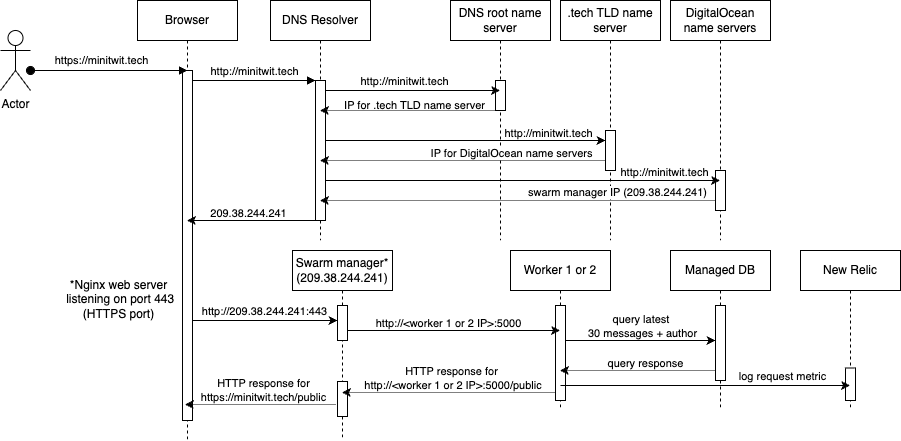
\includegraphics[width=\textwidth]{images/devops-sequence.png}
    \caption{The figure shows a sequence diagram describing a HTTP GET request to "minitwit.tech". }
    \label{fig:sequence}
\end{figure}


\begin{figure}[H]
    \centering
    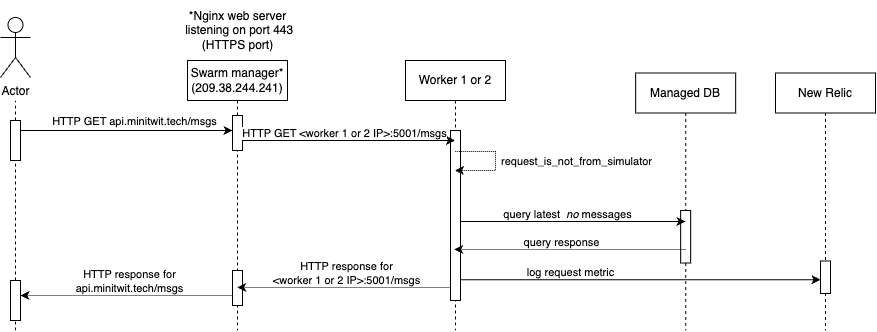
\includegraphics[width=\textwidth]{images/api-sequence.png}
    \caption{The figure shows a sequence diagram describing a HTTP GET request to "api.minitwit.tech/msgs". It is assumed that the \texttt{request\_is\_not\_from\_simulator} returns false. Otherwise it would return immediately with status code 403.}
    \label{fig:sequence_api}
\end{figure}


\subsection{Current state}
\todo{Describe the current state of your systems, for example using results of static analysis and quality assessments.}
SonarCloud and CodeClimate has been used for static analysis and quality assessment. 

Quality gate status on SonarCloud is passed and there are no issues and no security hotspots detected. The duplication of code is 1.7\& which is below the . It should be mentioned that the test files has been excluded from the static analysis because ... 


\section{Process' perspective}
\todo{This perspective should clarify how code or other artifacts come from idea into the running system and everything that happens on the way.
In particular, the following descriptions should be included:}
The project was developed using GitHub for version control and project management, using the Issues feature to track development tasks.


\subsection{CI/CD chain}
\todo{A complete description of stages and tools included in the CI/CD chains, including deployment and release of your systems. }
Our CI/CD chain is built using GitHub Actions. We have implemented workflows to automate testing, release and deployment of our code. We also use third-party tools as steps, including Dependabot and SonarCloud for static analysis.

\subsubsection{Automatic testing}
When a pull request is opened on GitHub, the \texttt{automatic-testing} workflow is triggered. This workflow builds a Docker image with the branch code, and runs it as an image using our \texttt{docker-compose} configuration. The workflow then runs the Python-based integration tests against this Docker container, and reports if any tests fail. 

\subsubsection{Deployment workflows}
We have two different deployment workflows that are somewhat similar but with different targets. The first is manually triggered only and deploys to a staging environment, used to test small features or changes. However, once we switched to a swarm setup, this environment was no longer used. In general, this works similar to the production deployment workflow, but targets the correct environment and tags the Docker image with the git commit's SHA-value instead.\\
The main deployment workflow runs on every push to the main branch, which checks out the code and logs in to \texttt{Docker Hub}. The workflow then builds the docker image, tagging it \texttt{latest} and pushes the image to Docker Hub, making it easy to pull and build this production-ready Docker image. The last action of the workflow is to establish an \texttt{ssh} connection to the swarm manager from which it runs our deploy script.\\
Once \texttt{deploy.sh} runs on the manager node, it sets the necessary environment variables in order to connect to the managed database, log to NewRelic and pull the correct image from Docker Hub before using \texttt{Docker Swarm's} command to execute a rolling deployment of the new Docker image. The \texttt{./remote\_files/docker-compose.yml} file is responsible for configuring the Docker swarm, such that there is a single replica for the frontend application whereas three replicas exists for the API that the simulator uses.\\

\subsubsection{Release workflow}
A simple workflow exists to ensure automatic releases are created on GitHub every time new code is added to the main branch. This workflow simply uses the two actions \texttt{actions/checkout@v4} and \texttt{actions/create-release@v1} to create a release with a version tag and release name based on the commit's SHA-value.

\subsubsection{Report workflows}
To ensure our report in our repository is always up to date, we utilise a built-in synchronization between Overleaf and GitHub. Once changes are made that a group member wish to save, one click from within Overleaf synchronizes the contents to a separate repository in our GitHub organisation, which triggers two Github Actions workflows:
\begin{enumerate}
    \item A workflow from within this report repository that notifies our main repository of any changes made to our report repository.
    \item A workflow from within the main repository that is called by the previously mentioned workflow, which triggers a git submodule update and commits it to the repository.
\end{enumerate}

\subsection{Monitoring \& Logging}
\todo{How do you monitor your systems and what precisely do you monitor?}
Both monitoring and logging of this project is done using New Relic. By installing the new relic agent on our VMs, and the new relic gem in our ruby application we can link it to the web interface. 
\\From here we can monitor A lot of metrics, but most importantly:
\begin{itemize}
    \item Web transaction time by application layer (See \ref{fig:transaction-times})
    \item Throughput for the application (Requests per minute) 
    \item The slowest transactions, by average response time.
    \item Error rate of transactions
\end{itemize}
Additionally we've set new relic up to send us alerts on slack, should the application suddenly have a significantly lower application throughput than usual, or if the error rate rises.
\begin{figure}[H]
    \centering
    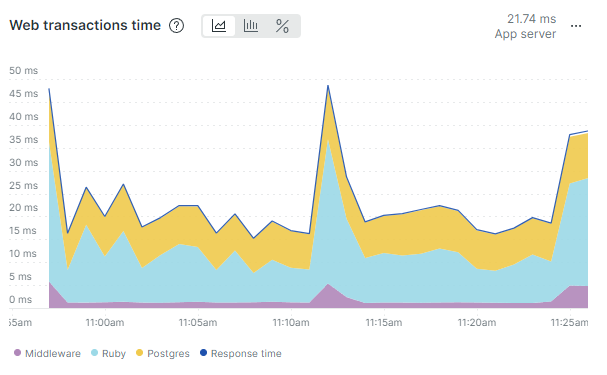
\includegraphics[width=\textwidth]{images/new-relic-transactions.png}
    \caption{The newrelic graph depicting web transaction times by application layer}
    \label{fig:transaction-times}
\end{figure}


\todo{What do you log in your systems and how do you aggregate logs?}
% NewRelic er begge dele

\subsection{Security}
\todo{Brief results of the security assessment and brief description of how did you harden the security of your system based on the analysis}

\subsection{Scaling and upgrading}
\todo{Applied strategy for scaling and upgrades}
% NB: Vi har skrevet lidt om det her i 2.1.2. Overvej om vi skal rykke noget derfra herned eller hvordan vi klarer det.

\subsection{Use of AI tools}
% \todo{In case you have used AI-assistants during your project briefly explain which system(s) you used during the project and reflect how it supported/hindered your process.}

In the beginning of the project, not all team members were familiar with the programming language Ruby. In order to get familiar, some of us had the Github Copilot extension enabled, allowing us to participate on a similar level as those who were more familiar with the language.\\

In the review process, ChatGPT has been used as a tool to interpret changes made by other members, by prompting ChatGPT to help understand the effects and consequences of the changes.\\

\section{Lessons learned perspective}
\todo{Describe the biggest issues, how you solved them, and which are major lessons learned with regards to: evolution and refactoring,
operation, and
maintenance 
of your ITU-MiniTwit systems. Link back to respective commit messages, issues, tickets, etc. to illustrate these. Also reflect and describe what was the "DevOps" style of your work. For example, what did you do differently to previous development projects and how did it work?}

\subsection{Evolution and refactoring}

\subsection{Operation}

\subsection{Maintenance}
% we used new relic to optimize code, using Apm to find missing indexes and such

\newpage
\section{Appendix}

\subsection{Development dependency graph} \label{appendix: dev-dependecies}
\begin{figure}[H]
    \centering
    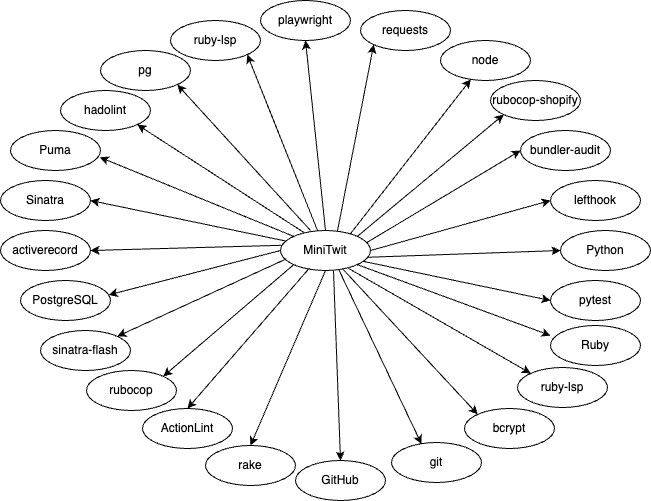
\includegraphics[width=\textwidth]{images/dependency-graph-dev.png}
    \caption{Development dependency graph.}
    \label{fig:dep-dev}
\end{figure}

\end{document}





